\ifdraft{\color{green}}{}\chapter{Fundamentação Teórica}

Para o entendimento e desenvolvimento da proposta conforme explícita nos objetivos gerais e específicos, alguns conceitos teóricos devem ser dispostos. Algoritmos do conceito ao modelo utilizado, variações de modelos algorítmicos e outros ambientes de estudo, ensino ou prática.

\section{Linguagem Natural}

Com menor rigidez do que se faz necessário para uma máquina, esses conjuntos também podem ser descritos em uma linguagem humanamente mais natural. Numa conversa ou em uma explicação de rota de um destino ou uma receita culinária o entendimento ocorrerá. Por depender de formalidade e buscando a aproximação com a rigidez das linguagens de programação utiliza-se o idioma estruturado. Em nosso caso o português estruturado, mas há também o inglês estruturado e certamente outras \ifdraft{\cite{citar}}{\cite{medina2006etal}}.

\section{Programas de Computador}

%\textrightarrow
Sua estrutura é E$\,\to\,$P$\,\to\,$S (entrada-programa-saída), podendo não haver argumentos de entrada. Exemplo, um programa após compilado pode receber em sua execução como argumento um número inteiro para resultar em sua raiz quadrada, ou outro sem receber argumento já tenha a raiz quadrada de um número pré definido \ifdraft{\cite{citar}}{\cite{medina2006etal}}.

\section{Pseudo código ou linguagem}

Visando ser uma ponte entre a linguagem natural e as linguagens de programação temos as pseudo-linguagem. Notadamente Portugol é evidenciada como a solução, pois desde \citeonline{saliba1992} é confirmada sua ampla utilização. Porém não há uma padronização existindo inúmeras variações, no entanto com muitas semelhanças entre si \ifdraft{\cite{citar}}{\cite{medina2006etal}}.

\section{Algoritmos}

A última das notas de Ada Lovelace, que foram republicadas em 1953\nocite{1253887}, apresenta os
primeiros conceitos sobre programação, descrevendo um algoritmo. Desde então
estes foram difundidos, sendo utilizados até a atualidade
\cite{santiago2003etal}.

Conforme \citeonline{medina2006etal} algoritmo é um termo mais amplo, sendo inclusive destinado a outras áreas e finalidades além da programação. As encontradas na literatura são interpretativas porém todas chegam ao mesmo resultado, um {\bfseries conjunto de instruções para a resolução de uma situação}.

Como algoritmo é um conjunto de instruções pode-se dizer então que ele é também um programa de computador, apresentando um conjunto de operações e instruções específicas para a saída que se pretende \cite{medina2006etal}.

%Alguns autores afirmam que estas instruções mas afirmações são determinam instruções são passos detalhadas para a solução ou mesmo que tipo de situação, se especificamente um problema ou tarefas em geral.

%Como podemos perceber, um programa nada mais é que um tipo de algoritmo. Sua particularidade é que suas operações são específicas para o computador e restritas ao conjunto de instruções que o processador pode executar. Podemos considerar esse conjunto de instruções como a primeira linguagem de programação do computador, também chamada de linguagem de máquina.

Para \citeonline{santiago2003etal} a estruturação do algoritmo com suas representações é dada da seguinte forma:

\begin{itemize}

\item Tipos de Dados: tipo de valores inserido nas variáveis;
\item Variáveis: armazenagem na memória principal;
\item Atribuições: definir valor numa variável;
\item Operações aritméticas: utilizadas em cálculos entre números e variáveis;
\item Estruturas de Controle: para fluxo, com desvio condicional e laços de repetição;
\item Operações relacionais: estabelecem relação entre comparações;
\item Vetores: variáveis com único nome, contendo um índice de posições.

\end{itemize}

% Com base nos dois parágrafos abaixo, reescrever utilizado como referência de embasamento os autores \cite{santiagodazzi2003}

%Um algoritmo consiste em um procedimento, composto por uma série de passos
%utilizados para resolver problemas computacionais específicos, que a partir do
%processamento comdados de entradas irá gerar dados de saídas (CORMEN et al,
%1999).

%Para efetuar funcionalidade em um algoritmo e verificar a integridade deste é
%necessário testar o algoritmo verificando o conteúdo das variáveis passo a
%passo. Para efetuar esta tarefa costuma-se utilizar o Teste de Mesa. Também
%chamado Teste Exaustivo, executa para cada instrução, uma verificação, e a
%amostragem do conteúdo das variáveis utilizadas no algoritmo, permitindo que o
%programador visualize o comportamento de todo o processo. Isso permite não
%apenas a comprovação do correto funcionamento, mas também detectar e corrigir
%com facilidade eventuais erros.

\section{Tradutores}
%Compiladores e Interpretadores

%Um compilador traduz um programa descrito em uma linguagem de alto nível, mais
%adequada aos seres humanos, para os códigos em uma linguagem de máquina, que
%podem ser executados por um processador. Grosso modo, o processo de
%compilação pode ser descrito como contendo as seguintes etapas: análise léxica, análise
%sintática, análise semântica e geração de código.\cite{barbosa2009etal}

Neste caso tradutor é um programa com capacidade de fazer leitura em uma linguagem e traduzir para outra equivalente. Conforme  \citeonline{aho2006etal} existem dois principais tipos de tradutores: compiladores (figura X)[p.~16]{medina2006etal} e interpretadores (figura X)[p.~17]{medina2006etal}. Ilustradas suas diferenças nas figuras referenciadas o interpretador é executado resultando na tradução direta das intruções passo a passo \cite{citar}

Passando por um processo de entendimento de elementos mínimos no código, ignorando outros e agrupando em símbolos especificados, a compilação se inicia. Além dessa análise também é necessária a verificação se esses grupos estão em ordem ou outros erros possíveis. \citeonline{citar} descreve que código fonte de entrada termina tendo como saída o programa objeto, o compilador converte a linguagem simples em uma linguagem entendida pela máquina.

Passando por um processo de entendimento de elementos mínimos no código, ignorando outros e agrupando em símbolos especificados, a compilação se inicia. Além dessa análise também é necessária a verificação se esses grupos estão em ordem ou outros erros possíveis. \citeonline{citar} descreve que código fonte de entrada termina tendo como saída o programa objeto, o compilador converte a linguagem simples em uma linguagem entendida pela máquina. Explicado o processo do compilador de maneira simples e objetiva é preciso ainda nomear tecnicamente além de expor sua etapas, sendo suas principais as análises: Léxica, Sintática e Semântica.

\begin{figure}[h]
  \caption{\ifdraft{\color{green}}{}Etapas de um compilador}\label{fig:compilador}
  \centering
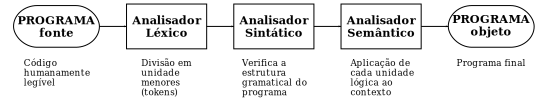
\includegraphics[width=\textwidth,height=10cm,keepaspectratio]{figures/etapas-compilador.pdf}
  \caption*{\ifdraft{\color{green}}{}\footnotesize Fonte: Autor, adaptado de \citeonline{ferrandin2005etal}.}
\end{figure}

%\subsection{Análise Morfológica}
%
\subsection{Análise Léxica}

Também denominada \textit{scanner} é onde elementos mínimos, \textit{tokens}, são identificados. Cada letra, número e outros caracteres (como pontuação e demais símbolos)  além do espaço após reconhecidos são então agrupados com lexemas em: palavras reservadas, comandos, conjunto de texto, nome de variáveis, inícios e fins do algoritmos ou de blocos nele

%\subsection{Tokenização e Parseamento}

\subsection{Análise Sintática}

Esses lexemas devem estar numa ordem que tenha sentido para sua execução correta.

%\subsection{Análise Semantica}

\section{Ferramentas Existentes}
% Ferramentas para prática de algoritmos

\begin{itemize}

\item \textbf{Construtor}: Desenvolvido pelo Centro Educacional de Informática Aplicada do SENAC (Rio de Janeiro), é a primeira ferramenta encontrada para uso em plataforma Windows e tem a vantagem acompanhar o livro ``Construção de Algoritmos`` de \citeonline{fernandes1999etal}.

\item \textbf{VisuAlg}: Desenvolvida por Claudio Morgado de Souza profissional programador e analista bem como professor universitário, é utilizada tanto em cursos técnicos quanto em meio universitário. A facilidade de obtenção do seu executável para Windows (não necessária instalação), documentação e simplicidade, sem perder funções úteis para iniciantes, são grandes atrativos \cite{souza2013etal}.

\item \textbf{Web Portugol}: Desenvolvida por pesquisadores na UNIVALI permite o acesso via navegadores que tenham integração com Java, desde que o mesmo também esteja instalado no computadors \cite{souza2013etal}.

\end{itemize}

Abaixo um comparativo de pontos que ressaltam como fatores determinantes em escolha da opção ao uso.

\begin{quadro}[h]
\centering
  \caption{Comparativo das ferramentas}\label{qua:compare-tools}
\begin{tabular}{| r | l | l | l | l |}\hline
& VisuAlg & Web Portugol & Portugol/Plus & Contrutor \\ \hline
Plataforma & Windows & Web (Java Applet) & DOS & Windows \\ \hline
Licença & \textit{freeware} & \textit{open source} & \textit{open source} & \textit{open source} \\ \hline
Instituição &  & UNIVALLI & UNOESC & SENAC \\ \hline
Linguagem &  & Java &  &  \\ \hline
\end{tabular}
  \caption*{\ifdraft{\color{green}}{}\footnotesize Fonte: Produção do autor.}
\end{quadro}

Desenvolvida por \citeonline{esmin1998} quando vinculado a UNOESC o \textbf{Portugol/Plus} é a mais antiga opção encontrada no Brasil. Merecendo destaque por ser comumente referenciada por outros autores inclusive quando tratam sobre desenvolvimento de novas soluções. Porém por ser em plataforma \textit{Disk Operating System (DOS)}, inclusive com interface gráfica foi desconsiderada no levantamento acima.

Ao delimitar a quantidade de itens outras também não foram listadas, alguns casos o acesso ao programa para testes não estava disponível ou menor relevância na literatura. No entanto  merecem menção: PascalX, por Athur Vargas Lopes da ULBRA; \textbf{Web-UNERJOL}\nocite{ferrandin2015}, utilizando UNERJOL os dois por acadêmico na UNERJ com colaboração.
%PascalX\nocite{http://www.ulbra.tche.br/~avl/home.htm}

Outras mais não foram consideradas por fugirem do escopo ao utilizar robótica, jogos, foco em estrutura de dados ou similares: Guido VanRobot, Robot Prog, Kids Ruby, Fut Code, TBC-AED. Eram pretendidas somente ferramentas com pseudo-linguagem algorítmica em português, preferencialmente Portugol, partindo novamente do Editor UAL como referencial.
%TBC-AED: por pesquisadores da Universidade Federal de Lavras/Departamento de Ciências da Computação em Minas Gerais

\section{UAL - Ensino com Livro Texto}

O livro ``Introdução à programação: 500 algoritmos resolvidos'' tem um grande apelo por seu elevado número resoluções como seu título deixa claro. Isso motiva os educadores utilizarem como livro texto base de disciplinas de ensino de Lógica da Programação \cite{citar}.

Neste livro é relatado o desenvolvimento da Linguagem UAL em um trabalho desenvolvido na UNESA. Era basicamente compilador via linha de comando, desenvolvido em Haskel para linux. Ele foi posteriormente portado para sistema operacional proprietário mais popular, e para este recebeu um editor próprio Editor UAL \cite{citar}.

Todos os algoritmos propostos para execução computadorizada são impressos nesta sintaxe variante do Portugol. Porém acompanha uma mídia ótica que contém os exercícios nesta e também para a desenvolvida por \citeonline{evaristo2000} o Interpretador de Linguagem Algorítmica (ILA) \cite{citar}.

%\the\textwidth
%455.0pt
%\halftextwidth
%227.7pt
%\noindent
\begin{quadro}[h]
\centering
  \caption{Comparativo UAL e ILA}\label{qua:compare-ualila}
\begin{tabular}{| p{75mm} | p{75mm} |}\hline
\multicolumn{1}{|c|}{\textbf{Em UAL}} & \multicolumn{1}{|c|}{\textbf{Em ILA}} \\ \hline
\begin{lstlisting}[language=ual]
prog algoritmo11
  imprima "Aprendendo prog!!!";
fimprog
\end{lstlisting} &
\begin{lstlisting}[language=ila]
//prog algoritmo11
inicio
  limpar
  escrever "Aprendendo inicio!!!"
fim
\end{lstlisting} \\ \hline
\end{tabular}
  \caption*{\ifdraft{\color{green}}{}\footnotesize Fonte: Autor, a partir dos exemplos de \citeonline{lopes2002etal}.}
\end{quadro}

Todo o projeto está pautado neste algoritmo simplista, porém se nota a diferença nos blocos de início e fim do programa, além de somente em UAL ter o nome do mesmo (solucionado com uso de linha comentada) e o comando de limpeza somente necessário em ILA. As chamadas de escrita em tela também têm sua palavra reservada diferente. Nenhuma delas delimita o argumento por parênteses e UAL exige ponto e vírgula ao final. As duas não são sensíveis no uso de letras maiúsculas ou minúsculas nas palavras chaves \cite{citar}.

Sendo o escopo das apresentações na estruturas de um algoritmo o escopo da linguagem \cite[p.~22]{spallanzani2000etal}, há diferenças entre UAL e ILA também quando quanto sua abrangência. Não tendo a UAL estruturas como matrizes n-dimensionais, funções com ou sem passagem de parâmetros, novos comandos para tomada de decisões e controle de repetições, novos tipos de dados, conversores de tipos.

\ifdraft{}{
%\subsection{Ensino Aprendizagem}

% NOTE citar Teoria das Inteligências Múltiplas de Gardner

%\section{Pseudoliguagem e Portugol}


%
%
%
%
%
%\item G-Portugol
%
%\item Portugol IDE
%
%\item Portugol Studio
%
%\item ASA
%
%\item ATMUF
%
%\item AWTM
%
%\item AMBAP
%
%\item CIFluxProg
%
%\item RAFF
%
%\item SistLog
%
%\item Ambiente SICAS
%
%\item C-Tutur
%
%\item PL-Detective

%\end{itemize}

%\subsection{UAL e Editor UAL}

%\subsection{Demais Aplicativos}
%
%%\subsection{Plataforma Digitais de Ensino}
%\subsection{Ambiente Virtual de Aprendizagem - AVA}
%
%% NOTE Interactive Learning - Aprendizado Interativo {tonin2012etal}
%
%\subsubsection{Udacity}
%
%\subsubsection{Codeacademy}
%
%\subsubsection{SoloLearn}
%
%\subsubsection{Code School}
%
%\subsubsection{Kan Academy}
%
%\subsection{Programação em Blocos}
%
%\subsubsection{\textit{Blockly}}
%
%\section{\textit{Online Judge}}
%
%Sistema de Apoio a Competições de Programação é a denominação em português de
%\textit{Online Judge} por \citeonline{campos2004etal}, nomeado como BOCA.
%E mais recente foi desenvolvido por acadêmico da URI (Universidade Regional
%Integrada do Alto Uruguai e das Missões) com base nesse trabalho anterior o URI
%\textit{Judge Online} \cite{tonin2012etal}.
%
%\section{Tecnologias Web}
%
%\subsection{Linguagem de Marcação de Texto}
%
%\subsection{Liguagem de Programação para Web}
%
%\subsubsection{ECMAScript}
%
%\subsubsection{WebAssembly}
%
%\subsection{Navegadores Web}
%
%\subsection{Aprimoramentos para Uso \textit{Offline}}
}
